
\documentclass[11pt,compress,t,notes=noshow, xcolor=table]{beamer}
\usepackage[]{graphicx}\usepackage[]{color}
% maxwidth is the original width if it is less than linewidth
% otherwise use linewidth (to make sure the graphics do not exceed the margin)
\makeatletter
\def\maxwidth{ %
  \ifdim\Gin@nat@width>\linewidth
    \linewidth
  \else
    \Gin@nat@width
  \fi
}
\makeatother

\definecolor{fgcolor}{rgb}{0.345, 0.345, 0.345}
\newcommand{\hlnum}[1]{\textcolor[rgb]{0.686,0.059,0.569}{#1}}%
\newcommand{\hlstr}[1]{\textcolor[rgb]{0.192,0.494,0.8}{#1}}%
\newcommand{\hlcom}[1]{\textcolor[rgb]{0.678,0.584,0.686}{\textit{#1}}}%
\newcommand{\hlopt}[1]{\textcolor[rgb]{0,0,0}{#1}}%
\newcommand{\hlstd}[1]{\textcolor[rgb]{0.345,0.345,0.345}{#1}}%
\newcommand{\hlkwa}[1]{\textcolor[rgb]{0.161,0.373,0.58}{\textbf{#1}}}%
\newcommand{\hlkwb}[1]{\textcolor[rgb]{0.69,0.353,0.396}{#1}}%
\newcommand{\hlkwc}[1]{\textcolor[rgb]{0.333,0.667,0.333}{#1}}%
\newcommand{\hlkwd}[1]{\textcolor[rgb]{0.737,0.353,0.396}{\textbf{#1}}}%
\let\hlipl\hlkwb

\usepackage{framed}
\makeatletter
\newenvironment{kframe}{%
 \def\at@end@of@kframe{}%
 \ifinner\ifhmode%
  \def\at@end@of@kframe{\end{minipage}}%
  \begin{minipage}{\columnwidth}%
 \fi\fi%
 \def\FrameCommand##1{\hskip\@totalleftmargin \hskip-\fboxsep
 \colorbox{shadecolor}{##1}\hskip-\fboxsep
     % There is no \\@totalrightmargin, so:
     \hskip-\linewidth \hskip-\@totalleftmargin \hskip\columnwidth}%
 \MakeFramed {\advance\hsize-\width
   \@totalleftmargin\z@ \linewidth\hsize
   \@setminipage}}%
 {\par\unskip\endMakeFramed%
 \at@end@of@kframe}
\makeatother

\definecolor{shadecolor}{rgb}{.97, .97, .97}
\definecolor{messagecolor}{rgb}{0, 0, 0}
\definecolor{warningcolor}{rgb}{1, 0, 1}
\definecolor{errorcolor}{rgb}{1, 0, 0}
\newenvironment{knitrout}{}{} % an empty environment to be redefined in TeX

\usepackage{alltt}
\newcommand{\SweaveOpts}[1]{}  % do not interfere with LaTeX
\newcommand{\SweaveInput}[1]{} % because they are not real TeX commands
\newcommand{\Sexpr}[1]{}       % will only be parsed by R
\newcommand{\xmark}{\ding{55}}%


\usepackage[english]{babel}
\usepackage[utf8]{inputenc}

\usepackage{dsfont}
\usepackage{verbatim}
\usepackage{amsmath}
\usepackage{amsfonts}
\usepackage{amssymb}
\usepackage{bm}
\usepackage{csquotes}
\usepackage{multirow}
\usepackage{longtable}
\usepackage{booktabs}
\usepackage{enumerate}
\usepackage[absolute,overlay]{textpos}
\usepackage{psfrag}
\usepackage{algorithm}
\usepackage{algpseudocode}
\usepackage{eqnarray}
\usepackage{arydshln}
\usepackage{tabularx}
\usepackage{placeins}
\usepackage{tikz}
\usepackage{setspace}
\usepackage{colortbl}
\usepackage{mathtools}
\usepackage{wrapfig}
\usepackage{bm}
\usepackage{amsmath}
\usepackage{pifont}

\usetikzlibrary{shapes,arrows,automata,positioning,calc,chains,trees, shadows}
\tikzset{
  %Define standard arrow tip
  >=stealth',
  %Define style for boxes
  punkt/.style={
    rectangle,
    rounded corners,
    draw=black, very thick,
    text width=6.5em,
    minimum height=2em,
    text centered},
  % Define arrow style
  pil/.style={
    ->,
    thick,
    shorten <=2pt,
    shorten >=2pt,}
}

\usepackage{subfig}

% Defines macros and environments
\usepackage{../../style/lmu-lecture}


\let\code=\texttt
\let\proglang=\textsf

\setkeys{Gin}{width=0.9\textwidth}

\setbeamertemplate{frametitle}{\expandafter\uppercase\expandafter\insertframetitle}

\usepackage{bbm}
% basic latex stuff
\newcommand{\pkg}[1]{{\fontseries{b}\selectfont #1}} %fontstyle for R packages
\newcommand{\lz}{\vspace{0.5cm}} %vertical space
\newcommand{\dlz}{\vspace{1cm}} %double vertical space
\newcommand{\oneliner}[1] % Oneliner for important statements
{\begin{block}{}\begin{center}\begin{Large}#1\end{Large}\end{center}\end{block}}


%new environments
\newenvironment{vbframe}  %frame with breaks and verbatim
{
 \begin{frame}[containsverbatim,allowframebreaks]
}
{
\end{frame}
}

\newenvironment{vframe}  %frame with verbatim without breaks (to avoid numbering one slided frames)
{
 \begin{frame}[containsverbatim]
}
{
\end{frame}
}

\newenvironment{blocki}[1]   % itemize block
{
 \begin{block}{#1}\begin{itemize}
}
{
\end{itemize}\end{block}
}

\newenvironment{fragileframe}[2]{  %fragile frame with framebreaks
\begin{frame}[allowframebreaks, fragile, environment = fragileframe]
\frametitle{#1}
#2}
{\end{frame}}


\newcommand{\myframe}[2]{  %short for frame with framebreaks
\begin{frame}[allowframebreaks]
\frametitle{#1}
#2
\end{frame}}

\newcommand{\remark}[1]{
  \textbf{Remark:} #1
}


\newenvironment{deleteframe}
{
\begingroup
\usebackgroundtemplate{
\includegraphics[width=\paperwidth,height=\paperheight]{../style/color/red.png}}
 \begin{frame}
}
{
\end{frame}
\endgroup
}
\newenvironment{simplifyframe}
{
\begingroup
\usebackgroundtemplate{
\includegraphics[width=\paperwidth,height=\paperheight]{../style/color/yellow.png}}
 \begin{frame}
}
{
\end{frame}
\endgroup
}\newenvironment{draftframe}
{
\begingroup
\usebackgroundtemplate{
\includegraphics[width=\paperwidth,height=\paperheight]{../style/color/green.jpg}}
 \begin{frame}
}
{
\end{frame}
\endgroup
}
% https://tex.stackexchange.com/a/261480: textcolor that works in mathmode
\makeatletter
\renewcommand*{\@textcolor}[3]{%
  \protect\leavevmode
  \begingroup
    \color#1{#2}#3%
  \endgroup
}
\makeatother





\input{../../latex-math/basic-math.tex}
\input{../../latex-math/basic-ml.tex}

\newcommand{\titlefigure}{figure/sample-dgp-2d.pdf}
\newcommand{\learninggoals}{
\item Understand structure of tabular data in ML 
\item Understand difference between target and features 
\item Understand difference between labeled and unlabeled data 
\item Know concept of data-generating process}

\title{Introduction to Machine Learning}
% \author{Bernd Bischl, Christoph Molnar, Daniel Schalk, Fabian Scheipl}
\institute{\href{https://compstat-lmu.github.io/lecture_i2ml/}{compstat-lmu.github.io/lecture\_i2ml}}
\date{}

\begin{document}
\lecturechapter{ML-Basics: Data}
\lecture{Introduction to Machine Learning}

% ------------------------------------------------------------------------------

\begin{vbframe}{Iris data set}
Introduced by the statistician Ronald Fisher and one
of the most frequently used toy examples.
\begin{itemize}
\item Classify iris subspecies based on flower measurements.
\item 150 iris flowers: 50 versicolor, 50 virginica, 50 setosa.
\item Sepal length / width and petal length / width in [cm].
\end{itemize}

\begin{center}
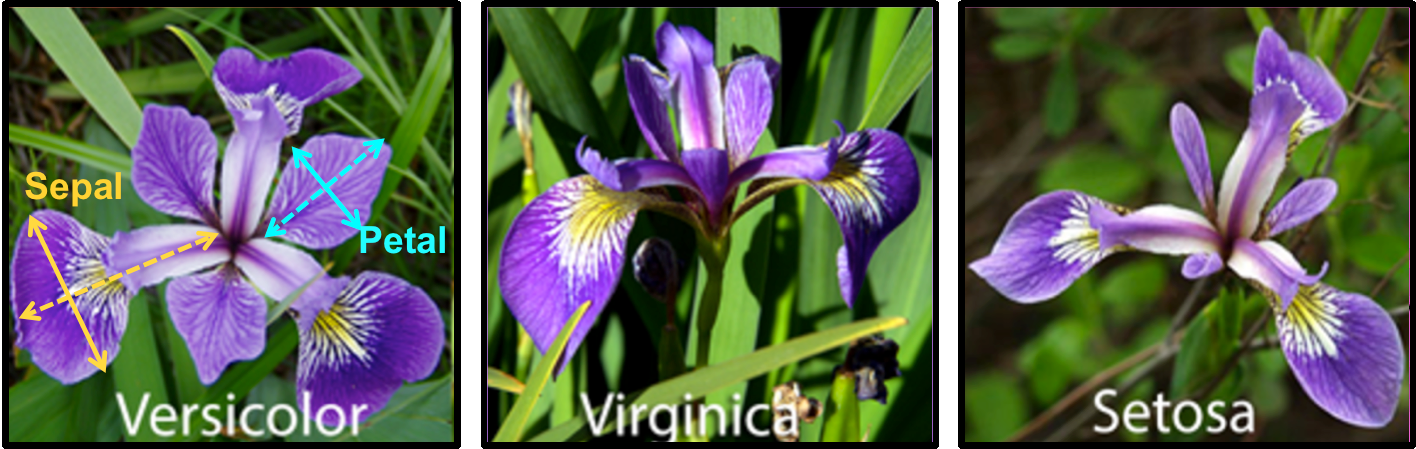
\includegraphics[width=0.9\textwidth]{figure_man/iris_species.png} 

\tiny
Source: \url{https://rpubs.com/vidhividhi/irisdataeda}
\normalsize
\end{center}

Word of warning: "iris" is a small, clean, low-dimensional data set,
which is very easy to classify; this is not necessarily true in the wild. 

\end{vbframe}

\begin{vbframe}{Data in Supervised Learning}

\begin{itemize}

  \item The data we deal with in supervised learning usually consists of 
  observations on different aspects of objects:
  
  \begin{itemize}
  
    \item \textbf{Target}: the output variable / goal of prediction

    \item \textbf{Features}: measurable properties that provide a concise 
    description of the object 
    
%    \item Both features and target variables may be of different data types  (categorical, numeric, ...)

  \end{itemize}
  
  \item We assume some kind of relationship between the features and the target,
  in a sense that the value of the target variable can be explained by a 
  combination of the features.
  
  % picturecreated with google presentation https://docs.google.com/presentation/d/1hoUHBJmXzCyVQXT9uP4sI84N6leQ42YhigFvQiCY0oo/edit?usp=sharing

    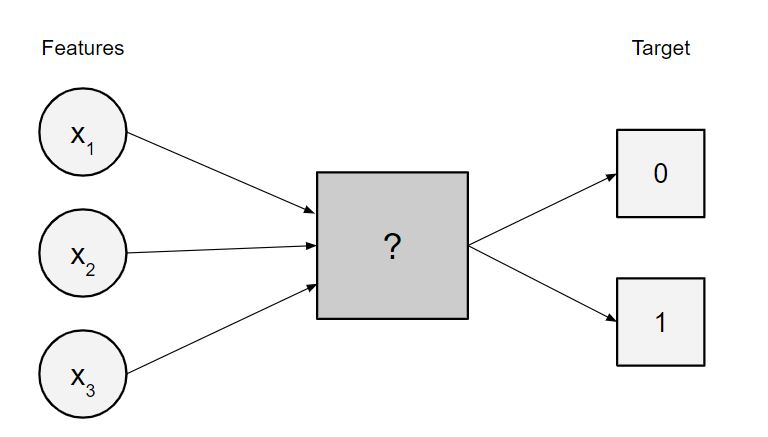
\includegraphics[width = 0.4\textwidth]{figure_man/feat_targ_rel.jpg}
     %picture created with google presentation
  %https://docs.google.com/presentation/d/1hnRPmCke8EqBhTrymC_pnuPe17Dk5iMkdBz6AQuIa3A/edit?usp=sharing page 1
    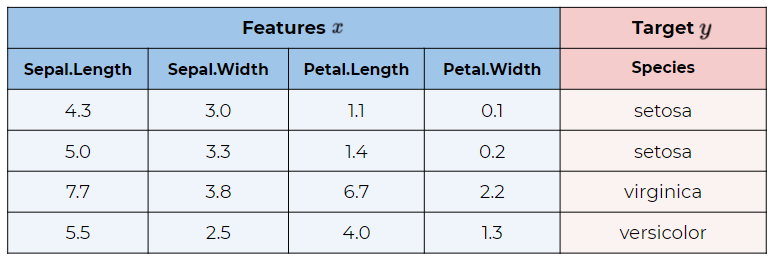
\includegraphics[width = 0.52\textwidth]{figure_man/ml-basic-data-example-iris.png} 

\end{itemize}

\end{vbframe}

% ------------------------------------------------------------------------------

\begin{vbframe}{Attribute types}

\begin{itemize}

  \item Both features and target variables may be of different data types 
  
  \begin{itemize}
  
    \item \textbf{Numerical} variables can have values in $\R$
    
    \item \textbf{Integer} variables can have values in $\Z$
    
    \item \textbf{Categorical} variables can have values in $\{C_1,...,C_g\}$
    
    \item \textbf{Binary} variables can have values in $\{0, 1\}$
  
  \end{itemize}
  
  \item For the \textbf{target} variable, this results in different tasks of supervised learning: \textit{regression} and \textit{classification}. 
  
  \item Most learning algorithms can only deal with numerical features,
      although there are some exceptions (e.g., decision trees can use integers and categoricals without problems).
      For other feature types, we usually have to pick or create an
      appropriate \textbf{encoding}, i.e., cast them to numerical values.
  \item If not stated otherwise, we assume numerical features.

\end{itemize}

\end{vbframe}


% ------------------------------------------------------------------------------

\begin{vbframe}{Encoding for categorical features}

\begin{itemize}
  \small
  % \item \textbf{Encoding} means transforming categorical features to numeric 
  % quantities.
  \item We expand the representation of a feature $x$
  with $k$ mutually exclusive categories from a scalar 
  %one to $\tilde k$ columns in the 
  %design matrix, each element being a \textbf{binary dummy variable} assuming 
  %values from \setzo.
  %\item $x$ is thus represented by 
  to a length-$\tilde k$ vector with at most one 
  element being 1, and 0 otherwise: $\bm{o}(x) = [\I(x = j)]_{
  j = 1, 2, \dots, \tilde k} \in \{0,1\}^{\tilde k}$.
  \item Each entry of $\bm{o}(x)$ is treated as a separate feature.
  \item Two popular ways to do this are
  \begin{itemize}
    \footnotesize
    \item \textbf{One-hot encoding}: $\tilde k = k$ dummies, so \textit{exactly 
    one} element is 1 (\enquote{hot}).
    E.g., $x \in \{ a, b, c\} \mapsto \bm{o}(x) = (x_a, x_b, x_c)$, with 
    $x_a = x_b = 0, x_c = 1$ and $\bm{o}(x) = (0, 0, 1)$ for $x = c$.
    \item \textbf{Dummy encoding}: $\tilde k = k - 1$ dummies, so 
    \textit{at most one} element is 1, cutting the redundancy of one-hot 
    encoding (necessary for learners that require non-singular input matrices, 
    such as in linear regression). \\
    E.g., $x \in \{ a, b, c\} \mapsto \bm{o}(x) = (x_a, x_b)$ for reference 
    category $c$, with $x_a = x_b = 0$ and $\bm{o}(x) = (0, 0)$ for $x = c$.
  \end{itemize} 
  \item For features with a natural \textbf{order} in their categories we 
  resort to encodings that reflect this ordinality, e.g., a sequence 
  of integer values.
  %-- note that equidistant values signify a linear ordering here.)
\end{itemize}

\end{vbframe}

% ------------------------------------------------------------------------------

\begin{vbframe}{Observation Labels}

\begin{itemize}

  \item We call the entries of the target column \textbf{labels}.
  \item We distinguish two basic forms our data may come in:
  
  \begin{itemize}
  
      \item For \textbf{labeled} data we have already observed the target
    
    \item For \textbf{unlabeled} data the target labels are unknown
  
  \end{itemize}
  
%  \item It is easy to see how labeled data are vastly more informative.
  
%  \item In practice, however, we will much more frequently encounter the unlabeled sort.
  
  \begin{center}
    %https://docs.google.com/presentation/d/1hnRPmCke8EqBhTrymC_pnuPe17Dk5iMkdBz6AQuIa3A/edit?usp=sharing page 2
    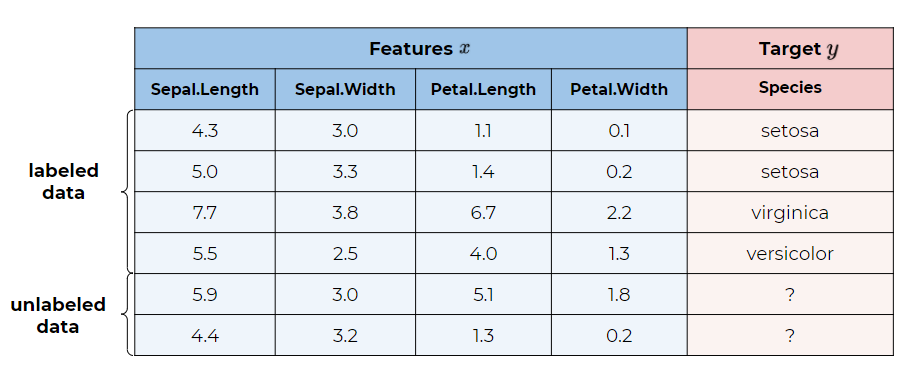
\includegraphics[width = 0.8\textwidth]{figure_man/ml-basic-data-example-iris-with-new.png} 
  \end{center}

\end{itemize}

\end{vbframe}

% ------------------------------------------------------------------------------

\begin{vbframe}{Notation for Data}

In formal notation, the data sets we are given are of the following form:
\[
\D = \Dset \in \defAllDatasetsn.
\]

We call

\begin{itemize}

  \item $\Xspace$  the input space with $p = \text{dim}(\Xspace)$ (for now: 
  $\Xspace \subset \R^p$),
  
  \item $\Yspace$ the output / target space,
  
  \item the tuple \(\xyi\) $\in \Xspace\times \Yspace$ the \(i\)-th observation,
  
  \item $\xj = \xjvec$ the j-th feature vector.
  
\end{itemize}

We denote

\begin{itemize}

  \item  $\defAllDatasetsn$, i.e., the set of all data sets of size $n$, as $\allDatasetsn$,
  \item $\defAllDatasets$, i.e., the set of all finite data sets, as $\allDatasets$.
\end{itemize}

\lz

So we have observed $n$ objects, described by $p$ features.

\end{vbframe}

% ------------------------------------------------------------------------------

\begin{vbframe}{Data-Generating Process}

\begin{itemize}

  \item We assume the observed data $\D$ to be generated by a process that can
  be characterized by some probability distribution $$\Pxy,$$ defined on 
  $\Xspace \times \Yspace$.
  
  \item We denote the random variables following this 
  distribution by lowercase $\xv$ and $y$.
  
  \item It is important to understand that the true distribution is essentially 
      \textbf{unknown} to us. In a certain sense, learning (part of) its structure is what ML is all about.
  
  \framebreak
  
  \item We assume data to be drawn \emph{i.i.d.} from the joint 
  probability density function (pdf) / probability mass function (pmf) $\pdfxy$.
  
  \begin{itemize}
  
    \item i.i.d. stands for \textbf{i}ndependent and \textbf{i}dentically 
    \textbf{d}istributed.
    
    \item This means: We assume that all samples are drawn from the same distribution 
    and are mutually independent -- the $i$-th realization does not depend on the
    other $n-1$ ones.
    
    \item This is a strong yet crucial assumption that is precondition to most
    theory in (basic) ML.
    % (e.g., the Central Limit Theorem).
    
  
  \end{itemize}

\end{itemize}

\begin{minipage}{0.5\textwidth}
  \centering
  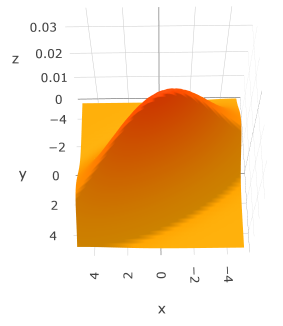
\includegraphics[width = 0.7\linewidth]{figure/sample-dgp-3d.png}
\end{minipage}%
\begin{minipage}{0.5\textwidth}
  % \centering
  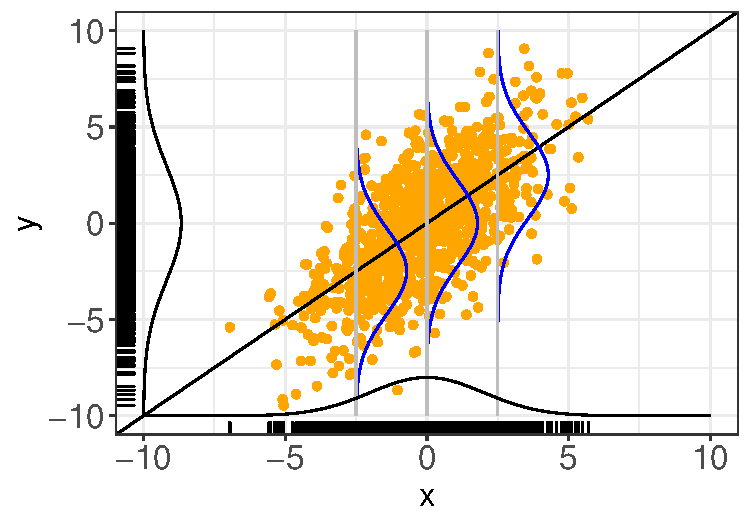
\includegraphics[width = 0.9\linewidth]{figure/sample-dgp-2d.pdf}
\end{minipage}

\framebreak

\textbf{Remarks:}

\begin{itemize}

  \item With a slight abuse of notation we write random variables, e.g., $\xv$ 
  and $y$, in lowercase, as normal variables or function arguments. The context 
  will make clear what is meant.
  
  \item Often, distributions are characterized by a parameter vector 
  $\thetab \in \Theta$. We then write $\pdfxyt$.
  
  \item This lecture mostly takes a frequentist perspective. Distribution 
  parameters $\thetab$ appear behind the | for improved legibility, not to imply 
  that we condition on them in a probabilistic Bayesian sense.
  So, strictly speaking, $p(\xv | \thetab)$ should usually be understood to mean 
  $p_{\thetab}(\xv)$ or $p(\xv, \thetab)$ or $p(\xv; \thetab)$.
  On the other hand, this notation makes it very easy to switch to a Bayesian view.

\end{itemize}

\end{vbframe}

% ------------------------------------------------------------------------------

\endlecture
\end{document}
